\documentclass[twocolumn]{IEEEtran}
\usepackage[utf8x]{inputenc}
\usepackage{amssymb,amsfonts}
\usepackage[tbtags]{amsmath}
\usepackage{graphicx}
\usepackage{cite}
\usepackage{slashbox}
\usepackage{pict2e}
\usepackage{float}
\usepackage[all]{xy}
\usepackage{graphics,graphicx,color,colortbl}
\usepackage{times}
\usepackage{subfigure}
\usepackage{wrapfig}
\usepackage{multicol}
\usepackage{cite}
\usepackage{url}
\usepackage[tbtags]{amsmath}
\usepackage{amsmath,amssymb,amsfonts,amsbsy}
\usepackage{bm}
\usepackage{algorithm}
\usepackage{algorithmic}
\usepackage[centerlast, small]{caption}
\usepackage[colorlinks=true, citecolor=blue, linkcolor=blue, urlcolor=blue,
breaklinks=true]{hyperref}

\begin{document}
\title{Respuesta en frecuencia (Resonancia)}
\author{José Fabio Lozano Ovalle Código: $222982$\\
	Wilson Orlando Macias Fuquen Código: $223101$\\
	David Ricardo Martínez Hernández Código: $261931$}
\maketitle
\markboth{Universidad Nacional de Colombia}{}
\floatname{algorithm}{Algoritmo}

\begin{abstract}
Se implementara un circuito $RLC$ serie que se encuentre en resonancia, teniendo en cuenta las condiciones de funcionamiento del generador de señales, se hallara la respuesta del circuito a la frecuencia midiendo valores experimentales de corriente y tensión para los elementos y finalmente se hallaran el ancho de banda y factor de calidad del circuito.
\end{abstract}

\begin{keywords}
Bobina, Condensador, Decibel, Energía, Frecuencia de Resonancia, Función de Transferencia, Ganancia, Resonancia.
\end{keywords}

\section{Objetivos}
\begin{itemize}
 \item Obtener una frecuencia de resonancia $\omega _0$ o $2*\pi f$, de acuerdo a los elementos utilizados en la práctica.
 \item Obtener la curva característica de un circuito $RLC$ en frecuencia, con un factor de calidad superior a $3$.
 \item Determinar el ancho de banda, la frecuencia de resonancia y el factor de calidad experimental del circuito $RLC$ serie.
\end{itemize}

\section{Introducción}
\noindent
El análisis de la respuesta en frecuencia es de gran importancia en el estudio de los fenómenos físicos, en este caso particular, los eléctricos, pues constituyen una base para comprender de una manera mejor conceptos como estabilidad o inestabilidad. También es de vital aplicación en el campo de las comunicaciones donde es necesario el diseño de dispositivos generadores y receptores, que puedan diferenciar entre determinados espectros frecuenciales. Es también utilizado en el diseño de sistemas de filtrado, sistemas de amplificación e innumerables aplicaciones. En resumen conocer el manejo de señales en el dominio frecuencia es una  herramienta matemática muy poderosa que nos ayuda a comprender mejor el estudio de las señales.

\section{Marco Teórico}
\noindent
\subsection{Función de Transferencia}
\noindent
La función de transferencia $H(\omega$ es usada como herramienta analítica para comprender la respuesta en frecuencia de un circuito. La función de transferencia de un circuito es el gráfico de la función de transferencia $H(\omega)$ contra $\omega$, con $\omega$ variando desde $\omega = 0$ hasta $\omega = \inf$.\\
La función de transferencia $H(\omega)$ de un circuito es la relación dependiente de la frecuencia de salida $Y(\omega)$ del fasor (un elemento de tensión o corriente) a una entrada del fasor $X(\omega)$ (fuente de tensión o corriente)\footnote{Definición tomada de \cite{sadiku}, Página 584}.\\
Una red lineal puede ser representado por el diagrama de bloques se muestra en la Fig. \ref{fig1}.
\begin{figure}[H]
	\centering
		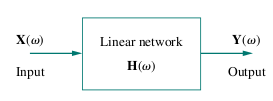
\includegraphics[scale=0.8]{bloquehs.png}
	\caption{Diagrama de bloque de una función de transferencia. (Figura tomada de \cite{sadiku}, Página 584)}
	\label{fig1}
\end{figure}
\noindent
Es decir
\begin{equation}
 H(\omega) = \frac{Y(\omega)}{X(\omega)}
\label{ecu1}
\end{equation}
\noindent
suponiendo condiciones iniciales iguales cero. Desde la entrada y la salida puede ser de voltaje o corriente en cualquier lugar en el circuito, hay cuatro funciones de transferencia posible:
\begin{equation}
 H(\omega) = Ganancia\ de\ Voltaje = \frac{V_{o}(\omega)}{V_{i}(\omega)}
\label{ecu2}
\end{equation}
\begin{equation}
 H(\omega) = Ganancia\ de\ Corriente = \frac{I_{o}(\omega)}{I_{i}(\omega)}
\label{ecu3}
\end{equation}
\begin{equation}
 H(\omega) = Transferencia\ de\ Impedancia = \frac{V_{o}(\omega)}{I_{i}(\omega)}
\label{ecu4}
\end{equation}
\begin{equation}
 H(\omega) = Transferencia\ de\ Admitancia = \frac{I_{o}(\omega)}{V_{i}(\omega)}
\label{ecu5}
\end{equation}

\subsection{Resonancia en serie}
\noindent
La característica más prominente de la respuesta en frecuencia de un circuito puede ser el pico afilado (o pico de resonancia) mostrado en sus características de amplitud.\\
La resonancia ocurre en cualquier sistema que tenga un par complejo conjugado de los polos, es la causa de las oscilaciones de la energía almacenada de una forma a otra. Es el fenómeno que permite la discriminación de frecuencias en las redes de comunicaciones. La resonancia ocurre en cualquier circuito que tiene al menos un inductor y un condensador.\\
En electricidad la resonancia es una condición en un circuito $RLC$ en el que las reactancias capacitiva e inductiva son iguales en magnitud, lo que resulta en una impedancia puramente resistiva\footnote{Texto tomado de \cite{sadiku}, Página 601}.\\
Un circuito $RLC$ Fig. \ref{fig2} en el dominio de la frecuencia. La impedancia de entrada es:
\begin{figure}[H]
	\centering
		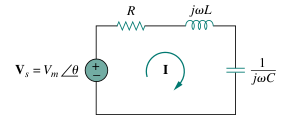
\includegraphics[scale=0.8]{circuitrlc.png}
	\caption{Circuito $RLC$ serie. (Figura tomada de \cite{sadiku}, Página 601)}
	\label{fig2}
\end{figure}
\begin{equation}
 Z = H(\omega) = \frac{V_s}{I} = R + j \omega L + \frac{1}{j \omega C}
\label{ecu6}
\end{equation}
\noindent o
\begin{equation}
 Z = R + j\left( {\omega L - \frac{1}{{\omega C}}} \right)
\label{ecu7}
\end{equation}
\noindent
La resonancia se genera cuando la parte imaginaria de la función de transferencia es igual a cero, o
\begin{equation}
 Im(Z) = \omega L - \frac{1}{\omega C} = 0
\label{ecu8}
\end{equation}
\noindent
El valor de $\omega$ que satisface esta condición es llamada \textit{frecuencia de resonancia $\omega _{0}$}, la condición de resonancia es
\begin{equation}
 \omega _{0} L = \frac{1}{\omega _{0} C}
\label{ecu9}
\end{equation}
\noindent o
\begin{equation}
 \omega _{0} =\frac{1}{\sqrt{LC}}\ rad/s
\label{ecu10}
\end{equation}
\noindent siendo $\omega _{0} = 2 \pi f_0$
\begin{equation}
 f_0 = =\frac{1}{2\pi \sqrt{LC}}\ Hz
\label{ecu11}
\end{equation}
\noindent
La respuesta en frecuencia de la magnitud de la corriente del circuito es
\begin{equation}
 I = \left| I \right| = \frac{{{V^m}}}{{\sqrt {{R^2} + {{\left( {\omega L - 1/\omega C} \right)}^2}} }}
\label{ecu12}
\end{equation}
\noindent
en la Fig. \ref{fig3} se encuentra ilustrado la simetría cuando el eje de la frecuencia se encuentra en escala logarítmica.
\begin{figure}[H]
	\centering
		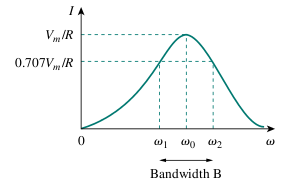
\includegraphics[scale=0.8]{ivsf.png}
	\caption{Amplitud de la corriente contra frecuencia en un circuito resonante. (Figura tomada de \cite{sadiku}, Página 602)}
	\label{fig3}
\end{figure}
\noindent
La medida de la potencia disipada por el circuito $RLC$ es
\begin{equation}
 P(\omega) = \frac{1}{12} I^{2} R
\label{ecu13}
\end{equation}
\noindent
La mayor potencia disipada se produce en resonancia, cuando $I = V_m / R$, de modo que
\begin{equation}
 P(\omega _0) = \frac{1}{12} \frac{V ^ {2}_{m}}{R}
\label{ecu14}
\end{equation}
\noindent
En ciertas frecuencias $\omega = \omega _1,\ \omega _2$, la potencia disipada es la mitad del valor máximo, es decir,
\begin{equation}
 P\left( {{\omega _1}} \right) = P\left( {{\omega _2}} \right) = \frac{{{{\left( {{V_m}/\sqrt 2 } \right)}^2}}}{{2R}} = \frac{{{V_m}^2}}{{4R}}
\label{ecu15}
\end{equation}
\noindent
Por lo tanto, $\omega _1$ y $\omega _2$ se llaman las \textbf{frecuencias de media potencia o half-power frequencies}.\\
Las frecuencia de media potencia se obtienen haciendo $Z$ igual a $\sqrt{2 R}$ y se escribe
\begin{equation}
 \sqrt {{R^2} + {{\left( {\omega L - \frac{1}{{\omega C}}} \right)}^2}}  = \sqrt 2 R
\label{ecu16}
\end{equation}
\noindent resolviendo la ecuación para $\omega$
\begin{equation}
 {\omega _1} =  - \frac{R}{{2L}} + \sqrt {{{\left( {\frac{R}{{2L}}} \right)}^2} + \frac{1}{{LC}}} 
\label{ecu17}
\end{equation}
\begin{equation}
 {\omega _2} =  \frac{R}{{2L}} + \sqrt {{{\left( {\frac{R}{{2L}}} \right)}^2} + \frac{1}{{LC}}} 
\label{ecu18}
\end{equation}
\noindent
Podemos relacionar las frecuencias de media potencia con la frecuencia de resonancia. A partir de las ecu. (\ref{ecu10}), (\ref{ecu17}) y (\ref{ecu18}),
\begin{equation}
 \omega _0 = \sqrt{\omega _1 \omega _2}
\label{ecu19}
\end{equation}
\noindent
A pesar de la altura de la curva de la Fig. \ref{fig3} está determinado por R, la anchura de la curva depende de otros factores. La anchura de la curva de respuesta depende del ancho de banda B, que se define como la diferencia entre las dos frecuencias de potencia media
\begin{equation}
 B = \omega _2 - \omega _1
\label{ecu20}
\end{equation}
\noindent
De manera rigurosa $B$ en la ecu. (\ref{ecu20}) es un ancho de banda de media potencia, ya que es el ancho de la banda de frecuencia entre las frecuencias de media potencia.\\
La efectividad de la resonancia en un circuito resonante es medido cuantitativamente por el \textit{factor de calidad \textbf{Q}}.
Esta resonancia es la energía reactiva en los circuitos oscilantes entre el inductor y el capacitor. La cualidad del factor hace referencia al máximo o la entrega de energía disipada en el circuito por ciclos de oscilación:
\begin{equation}
 Q = 2 \pi \frac{Pico\ de\ energia\ almacenada\ en\ el\ circuito}{Energia\ disipada\ por\ el\ circuito}
\label{ecu21}
\end{equation}
\noindent
Una medida de la energía estacionaria de un circuito en relación a esta energía disipada. En el circuito $RLC$ serie la energía estacionaria es $\frac{1}{2} L I^2$, cuando la energía disipada en un periodo es $\frac{1}{2} (I^2 R)(1/f)$, es decir
\begin{equation}
 Q = 2\pi \frac{{\frac{1}{2}L{I^2}}}{{\frac{1}{2}{I^2}R\left( {1/f} \right)}} = \frac{{2\pi fL}}{R}
\label{ecu22}
\end{equation}
\noindent o
\begin{equation}
 Q = \frac{\omega _0 L}{R} = \frac{1}{\omega _0 CR}
\label{ecu23}
\end{equation}
\noindent
Note que el factor de calidad es adimensional. La relacipon entre el ancho de banda $B$ y el factor de calidad $Q$ se obtiene sustituyendo la ecu. (\ref{ecu17}) y (\ref{ecu18}) en la ecu. (\ref{ecu20}) y utilizando al ecu. (\ref{ecu23}) se obtiene
\begin{equation}
 B = \frac{R}{L} = \frac{\omega _0}{Q}
\label{ecu24}
\end{equation}
\noindent o $B = \omega ^{2} _0 C R$. Es decir:\\
El factor de calidad $Q$  de un circuito resonante es el tiempo de esta frecuencia de resonancia a este ancho de banda\footnote{Definición tomada de \cite{sadiku}, Página 603}.\\
La Fig. \ref{fig4} el valor mas grande es el valor de $Q$, la selectividad del circuito es mayor pero es mas pequeño su ancho de banda. La selectividad de un circuito $RLC$ es la habilidad de respuesta del circuito a una frecuencias determinada y la discriminación a las demás frecuencias.
\begin{figure}[H]
	\centering
		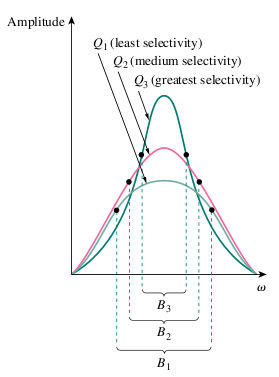
\includegraphics[scale=0.75]{resonancia.png}
	\caption{$Q$ contra ancho de banda. (Imagen tomada de \cite{sadiku}, Página 603)}
	\label{fig4}
\end{figure}
\noindent
Para que la banda de frecuencia rechace o acepte una frecuencia especifica es estrecha, el factor de calidad del circuito resonante debe ser alta. Si la banda de frecuencias es muy amplia, el factor de calidad debe ser bajo.\\
Se dice que es un circuito de alta $Q$ cuando su factor de calidad es igual o mayor que $10$. Para circuitos de alto-Q ($Q \geq 10$), las frecuencias de media potencia son, simétricas en torno a la frecuencia de resonancia y se puede aproximar como
\begin{equation}
 \omega _1 \simeq \omega _0 - \frac{B}{2}, \ \ \ \ \ \ \ \ \ \omega _2 \simeq \omega _0 + \frac{B}{2}
\label{ecu25}
\end{equation}

\subsection{Resonancia en paralelo}
\noindent
Un circuito  $RLC$ paralelo Fig. \ref{fig5}, es el dual de un circuito $RLC$ serie.
\begin{figure}[H]
	\centering
		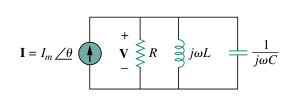
\includegraphics[scale=0.75]{rlcparalelo.png}
	\caption{Montaje del circuito $RLC$ paralelo. (Imagen tomada de \cite{sadiku}, Página 605)}
	\label{fig5}
\end{figure}
\noindent La admitancia es
\begin{equation}
 Y = H(\omega) = \frac{I}{V} = \frac{1}{R} + j \omega C + \frac{1}{j \omega L}
\label{ecu26}
\end{equation}
\noindent o
\begin{equation}
Y = \frac{1}{R} + j\left( {\omega C - \frac{1}{{\omega L}}} \right)
\label{ecu27}
\end{equation}
\noindent
La resonancia ocurre cuando la parte imaginaria de $Y$ es cero
\begin{equation}
 \omega C - \frac{1}{\omega L} = 0
\label{ecu28}
\end{equation}
\noindent o
\begin{equation}
 \omega _0 = \frac{1}{\sqrt{LC}}\ rad/s
\label{ecu29}
\end{equation}
\noindent
El voltaje $\left| V \right|$ de la Fig. \ref{fig6} Como función de la frecuencia.
\begin{figure}[H]
	\centering
		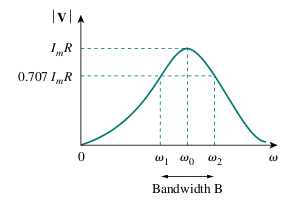
\includegraphics[scale=0.75]{parares.png}
	\caption{Amplitud de la corriente contra la frecuencia de resonancia del circuito $RLC$ paralelo. (Imagen tomada de \cite{sadiku}, Página 605)}
	\label{fig6}
\end{figure}
\noindent
Tenga en cuenta que en la resonancia, la combinación $LC$ en paralelo actúa como un circuito abierto, de modo que los flujos de las corrientes son todas a través de $R$. Además, el inductor y la corriente del condensador puede ser mucho más que el valor de fuente de corriente en resonancia.\\
Aprovechando la dualidad entre las Figs. \ref{fig2} y \ref{fig5} mediante la comparación de ecus. (\ref{ecu26}) con la ecu. (\ref{ecu7}). Mediante la sustitución de $R$, $L$ y $C$, en las expresiones para la conexión en serie con $ 1 / R $, $ 1 / C$, y $ 1 / L$ respectivamente, se obtiene para el circuito paralelo.
\begin{equation}
 {\omega _1} =  - \frac{1}{{2RC}} + \sqrt {{{\left( {\frac{1}{{2RC}}} \right)}^2} + \frac{1}{{LC}}} 
\label{ecu30}
\end{equation}
\begin{equation}
 {\omega _2} =  \frac{1}{{2RC}} + \sqrt {{{\left( {\frac{1}{{2RC}}} \right)}^2} + \frac{1}{{LC}}} 
\label{ecu31}
\end{equation}
\begin{equation}
 B = \omega _2 - \omega _1 = \frac{1}{RC}
\label{ecu32}
\end{equation}
\begin{equation}
 Q = \frac{\omega _0}{B} = \omega RC = \frac{R}{\omega _0 L}
\label{ecu33}
\end{equation}
\noindent
Utilizando las ecu. (\ref{ecu30}), ecu. (\ref{ecu31}) y ecu. (\ref{ecu33}), se puede expresar la potencia de frecuencia media en términos del factor de calidad, da como resultado:
\begin{equation}
 {\omega _1} = {\omega _0}\sqrt {1 + {{\left( {\frac{1}{{2Q}}} \right)}^2}}  - \frac{{{\omega _0}}}{{2Q}}
\label{ecu34}
\end{equation}
\begin{equation}
 {\omega _2} = {\omega _0}\sqrt {1 + {{\left( {\frac{1}{{2Q}}} \right)}^2}}  + \frac{{{\omega _0}}}{{2Q}}
\label{ecu35}
\end{equation}
\noindent Para $Q \geq 10$, se obtiene
\begin{equation}
 \omega _1 \simeq \omega _0 - \frac{B}{2}, \ \ \ \ \ \ \ \ \ \omega _2 \simeq \omega _0 + \frac{B}{2}
\label{ecu36}
\end{equation}

\section{Hipótesis}
\noindent
Se espera a que el voltaje se encuentre en fase con la corriente, debido a que las reactancias son iguales en magnitud, esto quiere decir que la reactancia total es cero y solo queda el valor resistivo. A demás se espera obtener un factor de calidad superior a $3$.\\
La reactancia del generador no debería influir en el comportamiento del circuito y el error obtenido debe ser pequeño.


\section{Materiales}
\begin{itemize}
 \item Bobina
 \item Condensador
 \item Generador de Señales
 \item Multímetro
 \item Osciloscopio
 \item Resistencias
\end{itemize}

\section{Análisis y Resultados Teóricos}
\noindent
Para esta práctica se implementara un circuito $RLC$, para el cual se analiza la respuesta en frecuencia y se calcula la frecuencia de resonancia.
\begin{figure}[H]
	\centering
		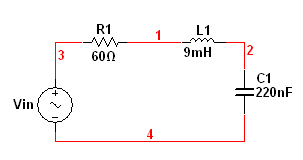
\includegraphics[scale=0.8]{circ1.PNG}
	\caption{Circuito RLC}
	\label{circ1}
\end{figure}
\noindent
Se tienen tres impedancias en serie las cuales son:
\begin{equation}
Z_R=R
\label{ecuR}
\end{equation}
\begin{equation}
Z_L=j \omega_0 L
\label{ecuL}
\end{equation}
\begin{equation}
Z_C =  \frac{1}{j\omega_0 C}
\label{ecuC}
\end{equation}
\noindent
Donde la impedancia total esta dada por
\begin{equation}
Z= R + j(\omega_0 L - \frac{1}{\omega_0 C})
\label{ecu101}
\end{equation}
\noindent
Para que $Z$ sea puramente real se debe cumplir que
\begin{equation}
\omega_0 L - \frac{1}{\omega_0 C}=0
\label{ecu102}
\end{equation}
\noindent
Despejando $\omega_0$ se tiene que la frecuencia de resonancia es
\begin{equation}
\omega_0=\sqrt{\frac{1}{LC}}
\label{ecu103}
\end{equation}
\noindent
Para el circuito de la Fig. \ref{circ1} se calcula una frecuencia de resonancia de
\begin{equation}
\omega_0=\sqrt{\frac{1}{(9mH)(0.22\mu F)}}=22473.328 Rad/seg
\label{ecu104}
\end{equation}
\noindent
\begin{equation}
f_0=\frac{\omega_0}{2 \pi}=\frac{22473.328Rad/seg}{2 \pi}=3576.741 Hz
\label{ecu104}
\end{equation}
\noindent
Con un factor de calidad
\begin{equation}
Q=\frac{L\omega_0}{R}=3.371
\label{ecu104}
\end{equation}
\noindent
Además  se tiene un ancho de banda
\begin{equation}
B=\frac{R}{L}=\frac{60\Omega}{9mH}=6666.67 Rad/seg=1061.0329 Hz
\label{ecu104}
\end{equation}

\section{Preguntas}
\begin{enumerate}
 \item ¿En que consiste el fenómeno de resonancia?\\
Es la condición que existe en un sistema físico cuando una función forzada de amplitud fija produce una respuesta de amplitud máxima, en el caso eléctrico se presenta este fenómeno cuando la impedancia de la red es puramente resistiva o mas exactamente cuando la reactancia se anula, como consecuencia tenemos que si una red esta en resonancia la tensión y la corriente en las terminales de entrada de la red están en fase.

 \item ¿Qué es Factor de calidad, ancho de banda y Frecuencia de resonancia ($F_o$)?\\
La frecuencia de resonancia es el valor que se necesita en un circuito para que se presente el fenómeno de resonancia, esto se debe a que en los elementos como capacitores e inductores las reactancias dependen directamente de la frecuencia.
\begin{equation}
 {F_0} = \frac{1}{{2\pi \sqrt {LC} }}
\label{ecu50}
\end{equation}
\noindent
El ancho de banda es el intervalo de frecuencias que comprende los valores de potencia media, también se puede calcular con la corriente del circuito, ya que sabemos que la corriente máxima se da en la frecuencia de resonancia y los valores de frecuencia que corresponden al $0.707$ de la corriente máxima son los mismos de la potencia media.
\begin{figure}[H]
	\centering
		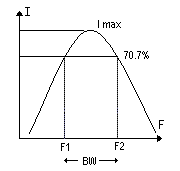
\includegraphics[scale=0.7]{figura1.png}
	\caption{Ancho de banda en función de la corriente}
	\label{figura1}
\end{figure}
\begin{equation}
 {B_\omega } = {F_2} - {F_1}
\label{ecu51}
\end{equation}
\noindent
El factor de calidad es la cantidad que se puede almacenar en un circuito, en comparación con la energía que se pierde durante un periodo completo de la respuesta. En términos de la frecuencia el factor de calidad $Q$ para un circuito $RLC$ serie es:
\begin{equation}
 Q = \frac{{2\pi {F_0}}}{{{B_\omega }}} = \frac{{2\pi {F_0}L}}{R}
\label{ecu52}
\end{equation}

 \item ¿Que sucede con la frecuencia de resonancia, el factor de calidad, y el ancho de banda
al variar independientemente $R$ o $L$ o $C$?\\
Para la frecuencia de resonancia si variamos R no se altera pero si cambiaos $L$ o $C$ habrá un cambio en esta. El factor de calidad depende de todos los valores porque un en $C$ cambiaría la frecuencia de resonancia vemos que el factor de calidad también depende de $L$ y $R$. El ancho de banda depende solamente de $R$ directamente y de $L$ de forma inversa, es decir aumenta cuando $R$ aumenta y disminuye cuando $L$ aumenta.

 \item ¿Cual es valor de la tensión $V_L + V_C$ en la práctica? ¿Concuerda con la teoría? Explique.\\
Esta pregunta se responderá en la práctica.

 \item ¿Que impacto tiene el generador de señales en la respuesta del sistema?\\
Como la Impedancia del generador es diferente de cero, también es susceptible de cambiar respecto a la frecuencia, a frecuencias muy grandes la componente inductiva  de la impedancia del generador será muy grande y frecuencias muy pequeñas la componente capacitiva es la que será considerable, entonces para algunos valores será grande la contribución en  determinada reactancia del generador a nuestro circuito.
\end{enumerate}

\bibliographystyle{ieeetran}
\begin{thebibliography}{99}
\bibitem{sadiku} Alexander, Charles K. \&  Sadiku, Matthew N.O.
{\em ```Fundamentals of Electric Circuits"'}.
McGRAW-HILL, ISE Editions, 1999.

\bibitem{dorf} Dorf  \& Svoboda.
{\em ```Circuitos Eléctricos"'}.
Alfaomega, Sexta Edición, 2006.

\bibitem{hayt} Hayt, William H. Jr., Kemmerly, Jack E. \& Durbin, Steven M.
{\em ```Análisis de circuitos en ingeniería"'}.
McGRAW-HILL, Séptima Edición, 2007.

\bibitem{nahvi} Nahvi, Mahmood \& Edminister, Joseph A.
{\em ```Theory and Problems of Electric Circuits"'}.
McGRAW-HILL, Fourth Edition, 2003.

\end{thebibliography}
\end{document}